\documentclass[titlepage]{jsreport}

\usepackage[dvipdfmx]{graphicx}
\usepackage{listings}
\usepackage{url}
\usepackage{bm}
\usepackage{cite}

% ソースコードを挿入するための設定
\lstset{
 	language = Python,
     frame = tbrl
}

\title{ガウス過程回帰を用いた効率的な相図探索}
\author{慶應義塾大学理工学部物理情報工学科\\
指導教員 渡辺宙志\\
学籍番号 61713173\\
内藤翔太}
\date{2020年MM月DD日}

\begin{document}

\maketitle

\tableofcontents

\chapter{はじめに} \label{chap:introduction}

「はじめに」もしくは「緒言」では、研究背景、目的、そして論文の構成を書く。

\section{研究の背景}

研究の背景は「なぜこの研究をしなければならないか」を、「大きい理由から小さい理由」へ書いていく。「大きい理由」は、「エネルギー問題」「安全」「便利」といった、「多くの人がほぼ納得するような理由」を挙げる。次に、その「大きな理由」を実現するために、これまでどのような試みがなされてきたかを説明する。これまでに読んだ論文のイントロダクションを参考に、必要な文献を引用しながら説得力のある文章を書くこと。

\section{研究の目的}

研究の背景を受けて、この研究分野は重要であるが、なんらかの不満点があることを述べる。その不満点は解決すべき問題であることを文献を引用しながら読者に納得させる。本研究の目的は、その不満点を解消することであることを述べ、その方法について簡単に述べる。

\section{本論文の構成}

論文の構成を説明する。まず本研究の目的を一行で書いてから、各章に何が書いてあるかを説明する。以下は例である。


本研究では、分野Aにおける手法Xの精度改善を行う。以下に本論文の構成を示す。第\ref{chap:introduction}章では、分野Aにおける手法の概観を紹介し、手法Xが広く用いられていることを示した。第\ref{chap:method}章では、本研究で用いる手法X、及びその改善手法であるX'について説明する。第\ref{chap:results}章では、本研究で提案した手法X'と、もととなった手法Xとの精度の比較を行う。第\ref{chap:summary}章では本研究で得られた知見を総括し、結論と今後の展望について述べる。




\chapter{手法} \label{chap:method}
\ref{method-sec:WCA-press}節ではWeeks-Chandler-Andersen\,(WCA)ポテンシャルにおける数密度と圧力の関係を調べる。
\ref{method-subsec:WCA}節ではWCAポテンシャルの説明を示し、
\ref{method-subsec:WCA-phase}節ではWCAポテンシャルの相図の概念図を示し、
\ref{method-subsec:WCA-pressure}節ではWCAポテンシャルにおける数密度と圧力の関係を調べる具体的な実験方法を示す。

\section{Weeks-Chandler-Anderse\,(WCA)ポテンシャルの圧力}\label{method-sec:WCA-press}


\subsection{Weeks-Chandler-Andersen\,(WCA)ポテンシャル}\label{method-subsec:WCA}
分子動力学計算において頻繁に用いられるモデルの一つにLennard-Jones\,(LJ)ポテンシャルと呼ばれるものが存在する。
LJポテンシャルは、アルゴンのような貴ガスのファンデルワールス力を記述するために提案\cite{Lennard_Jones_1931}されたもので、
このポテンシャルモデルにおいて二つの原子間相互作用ポテンシャルエネルギーは

\large
\begin{equation}
\phi(r)=4{\varepsilon}\left(\left(\frac{\sigma}{r}\right)^{12}-\left(\frac{\sigma}{r}\right)^6\right)\label{eq:lj}
\end{equation}
\normalsize
と表される。
ここで、rは原子間距離、${\sigma}$は原子直径の長さ、${\varepsilon}$はポテンシャルの深さを表す。
式(\ref{eq:lj})の右辺第一項は原子間の斥力相互作用を表し、右辺第二項は原子間の引力相互作用を表す。
LJポテンシャルを用いる系では、パラメータ$\sigma$\,,\,$\varepsilon$を用いて物理量を無次元化したLJ単位系と呼ばれる単位を用いる。
アルゴンでは、${\sigma}=3.40×10^{-10}\,\mathrm{m}$\,,\,${\varepsilon}=1.67×10^{-21}\,\mathrm{J}$であり\cite{argon-parameters}、
他にも多くの気体ごとに値が定められている\cite{graphane-parameters,many-parameters}。

LJ単位系では、温度$T^*$はポテンシャル$\varepsilon$\,,ボルツマン定数$k$を用いて、

\large
\begin{equation}
T^*=\frac{kT}{\varepsilon}\label{eq:T}
\end{equation}
\normalsize
圧力$P^*$はポテンシャル${\sigma}$\,,\,${\varepsilon}$を用いて

\large
\begin{equation}
P^*=\frac{P\sigma^3}{\varepsilon}\label{eq:P}
\end{equation}
\normalsize
数密度$\rho^*$はポテンシャル$\sigma$を用いて、

\large
\begin{equation}
\rho^*=\rho{\sigma}^3\label{eq:rho}
\end{equation}
\normalsize
と表される。

このLJポテンシャルの斥力作用と引力作用が入れ替わる$r=2^{\frac{1}{6}}{\approx}1.12246$にカットオフ距離を設けたポテンシャルをWCAポテンシャルと呼ぶ
(WCAポテンシャルでもLJ単位系を用いる)。
カットオフ距離とは、その距離内の原子間の相互作用のみを考慮するものであり、それ以上の距離での原子間の力を無視するものである\cite{WATANABE20191}。
WCAポテンシャルにおいて二つの原子間相互作用ポテンシャルエネルギーは、

\large
\begin{equation}
\phi(r) = \left\{ \begin{array}{ll}
    4{\varepsilon}\left(\left(\frac{\sigma}{r}\right)^{12}-\left(\frac{\sigma}{r}\right)^6\right) & (r\leq2^{\frac{1}{6}}) \\
    0 & (r>2^{\frac{1}{6}})\label{eq:wca}
\end{array} \right.
\end{equation}
\normalsize
と表される\cite{doi:10.1063/1.2176675}。
したがって、WCAポテンシャルとは式(\ref{eq:wca})のように斥力作用と引力作用が入れ替わる$r=2^{\frac{1}{6}}$にカットオフ距離を設けることにより、二原子間の引力作用を無視し、斥力作用のみを考慮したポテンシャルである。

以下の図{\ref{fig:dis-poen}にLJポテンシャルとWCAポテンシャルにおける原子間距離$r$と原子間のポテンシャルエネルギー$E$を示す。
(図{\ref{fig:dis-poen}ではLJポテンシャルにカットオフ距離2.5を設けている)

\begin{figure}[htbp]
    \begin{center}
        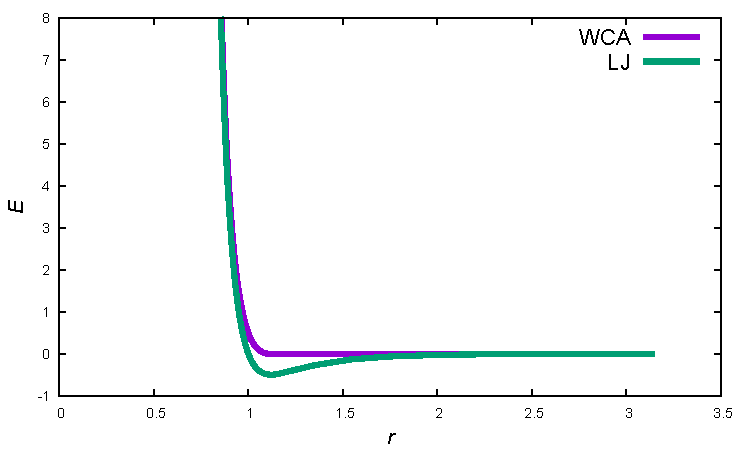
\includegraphics[width=13cm]{fig/dis-poen.pdf}
    \end{center}
    \caption{WCAとLJの原子間距離-ポテンシャルエネルギー}
    \label{fig:dis-poen}
\end{figure}
図{\ref{fig:dis-poen}に示すように、WCAポテンシャルはLJポテンシャルにカットオフ距離$r_c=2^{\frac{1}{6}}{\approx}1.12246$を設けることにより、
$r>r_c$でポテンシャルエネルギーが0になっている。


\newpage
\subsection{WCAポテンシャルの相図}\label{method-subsec:WCA-phase}
相図とは、熱力学的な状態量と物質や系の関係を表したものであり、相図の作成は、物性物理の分野において非常に重要である\cite{phase-diagram}。

以下の図\ref{fig:wca-phase-diagram}に式(\ref{eq:wca})に示したWCAポテンシャルの相図の概念図を示す。

\begin{figure}[htbp]
    \begin{center}
        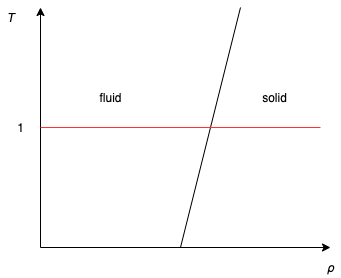
\includegraphics[width=9cm]{fig/wca-phase-diagram.png}
    \end{center}
    \caption{WCAポテンシャルの相図の概念図
    数密度、温度とWCAポテンシャルの相の関係を示す相図の概念図。
    \ref{method-subsec:WCA-pressure}節では赤線上の状態点($T^*$=1.0)を観測する。}
    
    \label{fig:wca-phase-diagram}
\end{figure}

図\ref{fig:wca-phase-diagram}に示すように、WCAポテンシャルはfluid(流体相)とsolid(固体相)の二相に分離する。
温度一定のまま密度を高くしていくと、ある密度で流体相から固体相への相転移を起こす。
この相転移近傍では、圧力の振る舞いが大きく変化するので、\ref{method-subsec:WCA-pressure}節では、
相転移近傍での圧力の振る舞いの変化を正しく捉えられるような手法を構築する。


\subsection{WCAポテンシャルの圧力測定}\label{method-subsec:WCA-pressure}
原子や分子の物理的な動きのコンピューターシミュレーション手法を分子動力学法(Molecular Dynamics method, MD)と言う\cite{molecular-dynamics}。
\ref{method-subsec:WCA-pressure}節では、式(\ref{eq:wca})に示したWCAポテンシャルにおける圧力の測定を分子動力学プログラムLarge-scale Atomic/Molecular Massively Parallel Simulator\,(LAMMPS)\cite{lammps}によるシミュレーションを用いて行う。
尚、本研究では、式(\ref{eq:wca})の${\sigma}$(原子直径の長さ)\,,\,${\varepsilon}$(ポテンシャルの深さ)を共に1.0とし、
図\ref{fig:wca-phase-diagram}で示した赤線上の状態点について、研究を進めるものとする。


本研究では、初期設定として1辺$L$の立方体の中に$N=2048$個の面心立方face-centered cubic\,(fcc)構造上に配置した分子を用意し、研究を進めるものとする。
以下の図\ref{initial-state-molecule}に、初期状態の分子構造を示す。

この系の数密度は、
\large
\begin{equation}
\rho = {\frac{N}{L^3}}{\label{eq:density}}
\end{equation}
\normalsize
と表される。

数密度$\rho=0.01$から15.0まで、0.01刻みで圧力$P$を測定した。圧力の測定にはLAMMPSを用いた。
この初期条件のもと、温度制御を1.0とし、タイムステップ0.001で20000実行のシミュレーションを行った。
尚、全ての研究でNVTによる温度制御ができていたことを前提とする。
NVTとは、

以下の図\ref{molecule-simulation}に、シミュレーション途中の分子構造を示す。


二体相互作用をする粒子系における圧力は、ビリアル定理によって

\large
\begin{equation}
PV=NkT+{\frac{1}{3}}\langle\sum_{i=j}^N\vec{q_{ij}} \cdot \vec{r_{ij}}\rangle{\label{eq:Theoritical-pressure}}
\end{equation}
\normalsize
と表される\cite{Theoritical-pressure,virial-therom}。
ここで、$P$は圧力、$V$は体積、$N$は原子数、$k$はボルツマン定数、$T$は温度、$\vec{q_{ij}}$は粒子iと粒子jの相対位置ベクトル、$\vec{r_{ij}}$は原子間に働く力ベクトルである。

\ref{method-subsec:WCA-phase}節に示したように、WCAポテンシャルはある密度で流体ー固体相転移を起こすことから、
相転移点近傍で圧力の振る舞いが急激に変化すると考えられる。
\ref{results-sec:WCA-press}節では、MDシミュレーションで測定されたWCAポテンシャルの圧力の振る舞いを、
原子間の相互作用をほぼ無視できる低密度状態、流体相から固体層への相転移近傍の中密度状態、原子間の相互作用の寄与が大きい高密度状態において調べる。

\section{WCAポテンシャルの状態方程式の推定}\label{method-sec:WCA-equation}
\ref{method-sec:WCA-equation}節では、\ref{results-sec:WCA-press}節で調べたWCAポテンシャルにおける圧力$P$を数密度$\rho$の状態方程式で表す。
\ref{method-subsec:virial}節、\ref{method-subsec:BWR}節では、それぞれ圧力を密度の項で展開するビリアル展開、Benedict-Webb-Rubin(BWR)方程式の説明を示し、
\ref{method-subsec:WCA-equation}節では、WCAポテンシャルの圧力を状態方程式で表す具体的な手法を示す。

\subsection{ビリアル展開}\label{method-subsec:virial}
気体の振る舞いを表す有望な記述の一つにビリアル展開と呼ぶものが存在する。
これは、Heikeによって1901年に提唱されたもの\cite{virial-Heike}で、多くの研究で利用されている\cite{virial-expansion-example1,virial-expansion-example2,virial-expansion-example3}。

理想気体の状態方程式は、

\large
\begin{equation}
P=RT{\rho} \label{eq:ideal-gas-virial}
\end{equation}
\normalsize
と表されるが、
実存気体の状態方程式のビリアル展開は、式(\ref{eq:ideal-gas-virial})にずれを補正する項を付け加えたもので、

\large
\begin{equation}
P=RT{\rho}+b_2{\rho}^2+b_3{\rho}^3+b_4{\rho}^4+\cdots \label{eq:virial}
\end{equation}
\normalsize
と表され、圧力$P$を密度$\rho$の冪級数を用いて表現する。
ここで、$T$は温度、$R$は気体定数である。
式(\ref{eq:virial})の密度$\rho$のn番目の累乗の係数を第nビリアル係数と呼ぶ\cite{virial-expansion}。
これらのビリアル係数は、増加する原子数で構成される集団群における原子の相互作用を表し、第2、第3、第4のビリアル係数は、2つ、3つ、4つ...の分子を含む衝突が気体中で重要になったときの理想的な振る舞いからの逸脱を表す。
高密度になるほど、多体の相互作用の寄与が大きくなるので、圧力が高くなるにつれて、考慮されなければならないビリアル項が増加する\cite{virial-Heike}。

\subsection{Benedict-Webb-Rubin(BWR)方程式}\label{method-subsec:BWR}
\ref{method-subsec:virial}節のように、Heikeが提唱したビリアル展開は、圧力を密度の冪級数を用いて表現したものであるが、この式に経験則的に指数の項を付け加えたものをBenedict-Webb-Rubin(BWR)方程式と呼ぶ。
BWR方程式は、軽質炭化水素の熱力学的性質を予測するために、1940年にManson、George、Rubinによって提唱された\cite{BWR-equation:original}。
BWR方程式の原式は、圧力$P$をモル密度$d$と絶対温度$T$の関数として表現したもので、

\large
\begin{equation}
P=RT{\rho}+\left(B_0RT-A_0-{\frac{C_0}{T^2}}\right){\rho}^2+(bRT-a){\rho}^3+{\frac{c}{T^2}}(1+{\gamma}{\rho}^2)e^{-{\gamma}{\rho}^2}{\rho}^3+a{\alpha}{\rho}^6\label{eq:BWR}
\end{equation}
\normalsize
と表される。

BWR方程式は、気体の状態方程式を表すことに概ね成功していたが、厳密には純粋な物質や混合物の熱力学的性質を予測するのに十分とは言えなかった。
そこで、1973年には、JacobsenとStewartによってBWR方程式の指数項をさらに増やした

\large
\begin{equation}
P=\sum_{n=1}^9a_n{\rho}^n+\exp(-{\gamma}{\rho}^2)\sum_{n=10}^{15}a_n{\rho}^{2n-17}\label{eq:mBWR}
\end{equation}
\normalsize
と表されるmodified-Benedict–Webb–Rubin(以下mBWR)方程式が提唱\cite{m-BWR-equation}されたが、
依然として気体の状態方程式を完璧に再現することは出来なかった。
その後も、多くの研究者が気体の状態方程式の項を増やすことで、完璧な再現を試みた\cite{MCCARTY1974276,BWR-equation:13,BWR-equation:25}が、項の個数は際限なく増え、項自体の物理的意味も不明瞭であった。

\subsection{WCAポテンシャルの状態方程式の推定}\label{method-subsec:WCA-equation}
\ref{method-subsec:virial}節、\ref{method-subsec:BWR}節のように気体の状態方程式を項を増やすことによって再現しようと試みたが、項の個数は際限なく増え続けた。
また、BWR方程式に含まれる指数項は経験的に付け加えられたものであり、物理的な意味が不明瞭である。

そこで、機械学習により、より多くの候補からWCAポテンシャルにおける状態方程式を推定する方が効果的であると言える。
最終的には、機械学習が推定してきた項の物理的意味を考察することが目標であるが、
まず本研究では\ref{results-sec:WCA-press}節で示したWCAポテンシャルにおける圧力と数密度の関係に上記で示した最小二乗法を適用し、
圧力を数密度に関する低次の多項式で近似することにより、WCAポテンシャルの状態方程式を推定する。

以下、最小二乗法の説明を簡潔に示す。
今、想定される多項式を

\large
\begin{eqnarray}
f(x)=\sum_{j=0}^m a_jx^j \nonumber
\end{eqnarray}
\normalsize
で表すとし、
測定で得られた、$x_i$\,,\,$y_i$の組を
\large
\begin{eqnarray}
\{(x_1,y_1)\,,\,(x_2,y_2)\,,\,\cdots\,,\,(x_n,y_n)) \}\nonumber
\end{eqnarray}
\normalsize
とすると、残差の二乗和$S$は、

\large
\begin{eqnarray}
S=\sum_{i=1}^n (y_i-f(x_i))^2\label{eq:residual-error}
\end{eqnarray}
\normalsize
と表され、これを最小にする$f(x)$を求めることで最小二乗法は実現される。


式(\ref{eq:residual-error})を行列表示にすると、

\footnotesize
\begin{eqnarray}
S = \left(
        \left[
            \begin{array}{c}
            y_1\\
            y_2\\
            \vdots\\
            y_n
            \end{array}
        \right]
        -
        \left[
            \begin{array}{cccc}
            x_1^m & x_1^{m-1} & \cdots & x_1^0 \\
            x_2^m & x_2^{m-1} & \cdots & x_2^0 \\
            \vdots & \vdots & \vdots & \vdots\\
            x_n^m & x_n^{m-1} & \cdots & x_n^0 \\
            \end{array}
        \right]
        \left[
            \begin{array}{c}
            a_m\\
            a_{m-1}\\
            \vdots\\
            a_0
            \end{array}
        \right]
    \right)^T
    \left(
        \left[
            \begin{array}{c}
            y_1\\
            y_2\\
            \vdots\\
            y_n
            \end{array}
        \right]
        -
        \left[
            \begin{array}{cccc}
            x_1^m & x_1^{m-1} & \cdots & x_1^0 \\
            x_2^m & x_2^{m-1} & \cdots & x_2^0 \\
            \vdots & \vdots & \vdots & \vdots\\
            x_n^m & x_n^{m-1} & \cdots & x_n^0 \\
            \end{array}
        \right]
        \left[
            \begin{array}{c}
            a_m\\
            a_{m-1}\\
            \vdots\\
            a_0
            \end{array}
        \right]
  \right)\nonumber
\end{eqnarray}
\normalsize
と表される。
ここで、
\large
\begin{eqnarray}
Y=  \left[
        \begin{array}{c}
        y_1\\
        y_2\\
        \vdots\\
        y_n
        \end{array}
    \right]\,,\,
X=  \left[
        \begin{array}{cccc}
        x_1^m & x_1^{m-1} & \cdots & x_1^0 \\
        x_2^m & x_2^{m-1} & \cdots & x_2^0 \\
        \vdots & \vdots & \vdots & \vdots\\
        x_n^m & x_n^{m-1} & \cdots & x_n^0 \\
        \end{array}
    \right]\,,\,
A=  \left[
        \begin{array}{c}
        a_m\\
        a_{m-1}\\
        \vdots\\
        a_0
        \end{array}
    \right] \nonumber
\end{eqnarray}
\normalsize
とすると、

\large
\begin{eqnarray}
S &=& (Y-XA)^T(Y-XA)\nonumber\\
  &=& Y^TY-2A^TX^TY+A^TX^TXA\label{eq:queue-residual-error}
\end{eqnarray}
\normalsize
と表され、$S$を最小化する$A$を求める最小二乗問題に帰着する。
最小二乗問題は

\large
\begin{eqnarray}
    {\nabla}S=\frac{\partial S}{\partial A}
    =
    \left[
        \begin{array}{c}
            \frac{\partial S}{\partial a_m}\\
            \frac{\partial S}{\partial a_{m-1}}\\
            \vdots\\
            \frac{\partial S}{\partial a_0}
        \end{array}
    \right]
    =
    \left[
        \begin{array}{c}
            0\\
            0\\
            \vdots\\
            0
        \end{array}
    \right]\label{eq:Least-squares-problem}
\end{eqnarray}
\normalsize
から得られる連立方程式を$A$について解くことで表され、式(\ref{eq:queue-residual-error})\,,\,式(\ref{eq:Least-squares-problem})より、

\large
\begin{eqnarray}
    {\nabla}S&=&-2X^TY+2X^TXA=0\nonumber\\
    &{\Leftrightarrow}&{\ }{\ }X^TXA=X^TY\nonumber\\
    &{\Leftrightarrow}&{\ }{\ }A=(X^TX)^{-1}X^TY\label{eq:normal-equation}
\end{eqnarray}
\normalsize
で与えられる$A$を求めることで最小二乗法は完結する\cite{least-squares}。

\ref{results-sec:WCA-equation}節では、上記で述べたように\ref{results-sec:WCA-press}節で示したWCAポテンシャルにおける圧力と数密度の関係に
上記で示した最小二乗法を適用し、圧力を数密度に関する低次の多項式で近似することにより、WCAポテンシャルの状態方程式を推定する。
その後、推定したWCAポテンシャルの状態方程式の展開係数が先行研究と矛盾しないことを確認する。


\section{Gaussian Process Regression(ガウス過程回帰)による効率的推定}\label{method-sec:Gauss}
\ref{method-sec:Gauss}節では、ガウス過程回帰を用いて、WCAポテンシャルの状態方程式を効率的に求める。
\ref{method-subsec:Gauss}節では、ガウス過程回帰の説明を示し、
\ref{method-subsec:Gaussian-estimation}節では、\ref{results-sec:WCA-press}節で示したWCAポテンシャルにおける数密度と圧力のペア($\rho$\,,\,$P$)の数点にガウス過程回帰を適用し、
WCAポテンシャルの数密度と圧力の関係を効率的に推定する具体的な方法を示す。


\subsection{ガウス過程回帰}\label{method-subsec:Gauss}
ガウス過程回帰は、出力の不確実性も定量化できる確率的な補間予測を提供する\cite{machine-learning}。


$N$個の観測値、すなわち入力$x$\,,\,$y$の$N$個のペア

\large
\[
    \mathcal{D}=\{(x_1,y_1)\,,\,(x_2,y_2)\,,\,\cdots\,,\,(x_N,y_N)\}
\]
\normalsize
が与えられているとし、$\bm{X}=(x_1,\cdots,x_N)$\,,\,$\bm{y}=(y_1,\cdots,y_N)$とする。
簡単のため、$y$は平均が$\bm{0}$となるように正規化してあるとし、$y=f(x)$という関数$f$が平均$\bm{0}$のガウス過程

\large
\begin{eqnarray}
    f\,{\sim}\,GP(\bm{0},k(x,x'))\nonumber
\end{eqnarray}
\normalsize
から生成されているとする。
尚、$k(x,x')$は、カーネル関数と呼ばれるもので入力$x$の間の類似度を測るために使われるものであり\cite{Gauss-machine-learning}、測定値間の入力$x\,,\,x'$から求められる。

ここで、
\large
\begin{eqnarray}
\bm{y}=  
    \left[
        \begin{array}{c}
        y_1\\
        y_2\\
        \vdots\\
        y_N
        \end{array}
    \right] \nonumber
\end{eqnarray}
\normalsize
とおけば、この$\bm{y}$はガウス分布に従い、入力のすべてのペア$(x_n,x_{n'})$についてカーネル関数
$k(x,x')$を用いて、

\large
\begin{eqnarray}
K_{nn'}
=   k(x_n,x_{n'})\nonumber
\end{eqnarray}
\normalsize
で与えられるカーネル行列$\bm{K}$を使って、

\large
\begin{eqnarray}
\bm{y}
\,{\sim}\,{\mathcal{N}}(\bm{0},\bm{K})  \nonumber
\end{eqnarray}
\normalsize
が成立する。

今、データに含まれない$\bm{X}^*=(x_1^*,\cdots,x_M^*)$での$\bm{y}^*=(y_1^*,\cdots,y_M^*)$の値を予測する。
$\bm{y}$に$\bm{y}^*$を含めたものを新しく

\large
\begin{eqnarray}
\bm{y'}=  
    \left[
        \begin{array}{c}
        y_1\\
        y_2\\
        \vdots\\
        y_N\\
        y_1^*\\
        y_2^*\\
        \vdots\\
        y_M^*\\
        \end{array}
    \right] \nonumber
\end{eqnarray}
\normalsize
とし、$\bm{X}$および、$\bm{X}^*$から計算される$(N+M)×(N+M)$次元のカーネル行列を$\bm{K'}$とすると、
これら全体がまたガウス分布に従うので、

\large
\begin{eqnarray}
\bm{y'}
\,{\sim}\,{\mathcal{N}}(\bm{0},\bm{K'})  \nonumber
\end{eqnarray}
\normalsize
が成立する。

つまり、ガウス過程回帰は、\cite{Gaussian-Processes-for-Machine-Learning}で開発された導出に従って、観測された$\bm{y}$と予測された$\bm{y}^*$の同時分布が

\large
\begin{eqnarray}
    \left[
        \begin{array}{l}
            \bm{y} \\
            \bm{y}^* 
        \end{array}
    \right]
    {\sim}\,{\mathcal{N}}
    \left(0,
        \left[
            \begin{array}{cc}
                \bm{K} & \bm{k}_*\\    
                \bm{k}_*^T & \bm{k}_{**}
            \end{array}
        \right]
    \right) \label{eq:Gaussian-distribution}
\end{eqnarray}
\normalsize
のようなガウス分布に従う。
尚、$\bm{K}$は測定値の入力$x$と$x'$から求められ、$\bm{k}_*$は測定値の入力$x$と測定されていない入力$x'^*$から求められ、
$\bm{k}_{**}$は測定されていない入力$x^*$と測定されていない入力$x'^*$から求められる。

このガウス過程の予測分布は、式(\ref{eq:Gaussian-distribution})から、

\large
\begin{eqnarray}
p(\bm{y}^*|\bm{x}^*,\mathcal{D})
={\mathcal{N}}(\bm{k}_*^T\bm{K}^{-1}\bm{y}\,,\,\bm{k}_{**}-\bm{k}_*^T\bm{K}^{-1}\bm{k}_*)  \label{eq:Gaussian-predicted-distribution}
\end{eqnarray}
\normalsize
と表わされる。
以上から、未知のデータは平均を$E$、分散を$\sigma^2$とすると

\large
\begin{eqnarray}
    E&=&\bm{k}_*^T\bm{K}^{-1}\bm{y}\\ \label{eq:Gaussian-predicted-average}
    \sigma^2&=&\bm{k}_{**}-\bm{k}_*^T\bm{K}^{-1}\bm{k}_* \label{eq:Gaussian-predicted-decentration}
\end{eqnarray}
\normalsize
を満たすようなガウス分布に従う\cite{Gauss-machine-learning}。

式(\ref{eq:Gaussian-predicted-distribution})に示すようなガウス分布に基づき、未知のデータを推定するが、
このガウス分布を元に次に評価する点を決定する必要が生じる。この際に、式(\ref{eq:Gaussian-predicted-decentration})の分散$\sigma^2$の関数として
「獲得関数」と呼ばれるものを使用する。
獲得関数とは関連分野から借りてきた試行状態の「情報性」を定量化する用語に過ぎない\cite{acquisition-function}。


\subsection{ガウス過程回帰によるWCAポテンシャルの状態方程式の効率的推定}\label{method-subsec:Gaussian-estimation}
\ref{method-subsec:Gauss}節に示したガウス過程回帰を用いて、本研究では、WCAポテンシャルにおける数密度$\rho$と圧力$P$の関係を効率的に推定する。

本研究では、カーネル関数として、\cite{Gauss-machine-learning}で導入されている

\large
\begin{eqnarray}
    k(x,x')=\theta_1\exp\left(-\frac{(x-x')^2}{\theta_2}\right)+\theta_3\delta(x,x')\\ \label{eq:Gauss-kernel}
    (\theta_1=1.0,\theta_2=0.4,\theta_3=0.1) \nonumber \\ 
    (x=x':\delta(x,x')=1) \nonumber \\
    (x\,{\neq}\,x':\delta(x,x')=0) \nonumber
\end{eqnarray}
\normalsize
を採用する。

\ref{results-sec:WCA-press}節に、数密度$\rho=\{0.00,0.01,0.02,\cdots,15.0\}$と圧力$P$の関係を示したが、全データのうち端点となる、
$\{(P,\rho)\}=\{(0.00,0.00)\,,\,(15.0,1.83×10^7)\}$の二点を初期の入力データとして、ガウス過程回帰を適用する。
式(\ref{eq:Gaussian-predicted-average})の平均$E$が入力データから予測される関数を、
式(\ref{eq:Gaussian-predicted-decentration})の分散$\sigma^2$が入力データから予測される関数の不確かさを示すものとする。
また、各数密度における分散の平方根を取った標準偏差$\sigma$の大きさを獲得関数とし、この関数を最大にする、すなわち不確かさが最大の数密度を次の試行点として選択する。
この数密度におけるWCAポテンシャルの圧力をMDシミュレーションにより測定し、入力データを更新し、

\chapter{結果} \label{chap:results}

\section{WCAポテンシャルの圧力}\label{results-sec:WCA-press}
\ref{results-sec:WCA-press}節では、各数密度においてMDシミュレーションで測定されたWCAポテンシャルの圧力の振る舞いを調べる。
まず、数密度$\rho$とMDシミュレーションで測定されたWCAポテンシャルの圧力$P$の関係を
以下の図\ref{fig:den-pre}に示す。

\begin{figure}[htbp]
    \begin{center}
        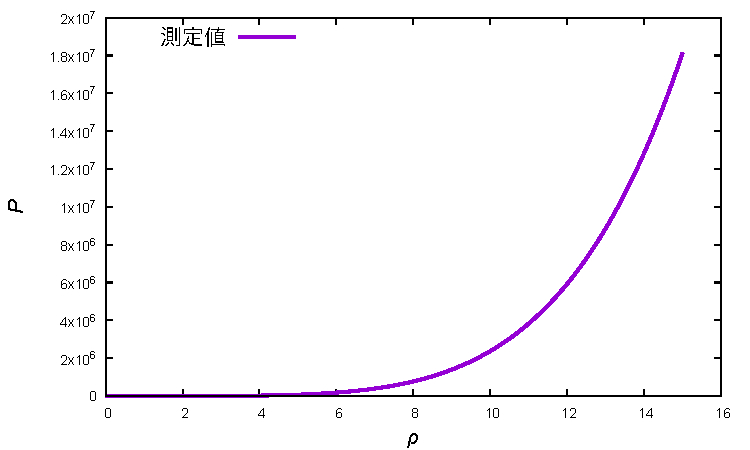
\includegraphics[width=14cm]{fig/den-pre.pdf}
    \end{center}
    \caption{WCAポテンシャルの圧力の測定値}
    \label{fig:den-pre}
\end{figure}

以下、\ref{results-subsec:WCA-press-low-density}節では原子間の相互作用をほぼ無視できる低密度状態、
\ref{results-subsec:WCA-press-middle-density}節では流体相から固体相への相転移近傍の中密度状態、
\ref{results-subsec:WCA-press-high-density}節では原子間の相互作用の寄与が大きい高密度状態において、
MDシミュレーションで測定されたWCAポテンシャルの圧力について具体的に調べる。


\subsection{低密度状態のWCAポテンシャルの圧力}\label{results-subsec:WCA-press-low-density}
初期状態において、原子間の相互作用が作用する($原子間距離r=カットオフ距離2^{\frac{1}{6}}{\approx}1.12246$)数密度は

\large
\begin{eqnarray}
\rho\,{\simeq}\,1.00 \nonumber
\end{eqnarray}
\normalsize
と表されるため、

\large
\begin{equation}
\rho\,{\leq}\,1.00 \label{eq:lowdensity-density}
\end{equation}
\normalsize
では、原子間の相互作用をほぼ無視できる。
上記の式(\ref{eq:lowdensity-density})を満たすような低密度状態における分子の状態の概念図を以下の図\ref{fig:lowdensity.png}に示す。

\begin{figure}[htbp]
    \begin{center}
        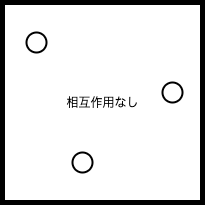
\includegraphics[width=6cm]{fig/lowdensity.png}
    \end{center}
    \caption{低密度状態における分子の状態の概念図}
    \label{fig:lowdensity.png}
\end{figure}

上図の図\ref{fig:lowdensity.png}のような低密度状態においては、原子間の相互作用をほとんど無視できるので、
圧力は式(\ref{eq:Theoritical-pressure})の第一項のみを用いて、
\large
\begin{equation}
PV\,{\simeq}\,NkT{\label{eq:ideal-gas}}
\end{equation}
\normalsize
と近似できる。


式(\ref{eq:ideal-gas})より、
\large
\begin{eqnarray}
PV\,&{\simeq}&\,NkT\nonumber\\
{\Leftrightarrow}{\ }{\ }P\,&{\simeq}&\,{\frac{N}{V}}kT\nonumber\\
{\Leftrightarrow}{\ }{\ }P\,&{\simeq}&\,{\rho}kT\nonumber
\end{eqnarray}
\normalsize
と書け、本研究では、$k=1$、$T=1$と設定し、MDシミュレーションにより圧力測定を行ったので、

\large
\begin{equation}
P\,{\simeq}\,{\rho} \label{eq:ideal-value}
\end{equation}
\normalsize
と表現できることが予測される。

式(\ref{eq:ideal-value})を「理論近似値」、本研究におけるMDシミュレーションにより測定された圧力を「測定値」とし、その結果を図\ref{fig:lowden_compare:den-pre}に示す。

\begin{figure}[htbp]
    \begin{center}
        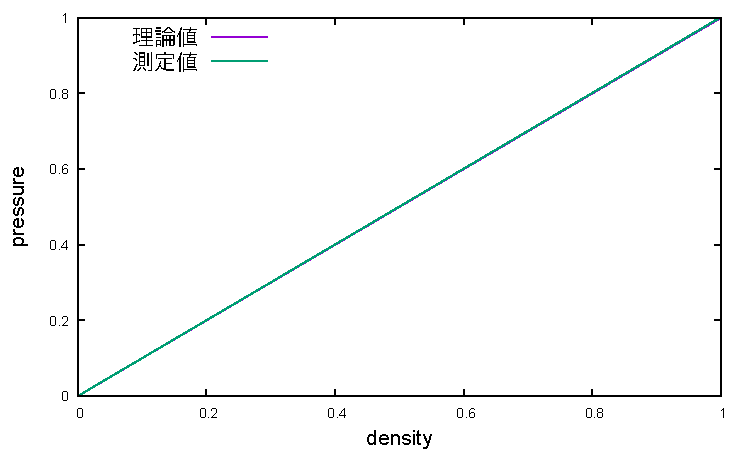
\includegraphics[width=14cm]{fig/lowden_compare:den-pre.pdf}
    \end{center}
    \caption{WCAポテンシャルにおける低密度状態の圧力の理論近似値と測定値の比較}
    \label{fig:lowden_compare:den-pre}
\end{figure}

図\ref{fig:lowden_compare:den-pre}から、低密度状態ではWCAポテンシャルの圧力は式(\ref{eq:ideal-gas})
と書けることがわかる。
これは、低密度状態では、「ほぼ」原子間の相互作用を無視でき、原子が理想気体のように振る舞うことに依存する。


\subsection{中密度状態のWCAポテンシャルの圧力}\label{results-subsec:WCA-press-middle-density}
中密度状態では、相互作用を持つ分子ペアと持たない分子が存在する。
まず、中密度状態における分子の状態の概念図を以下の図\ref{fig:middledensity.png}に示す。

\begin{figure}[htbp]
    \begin{center}
        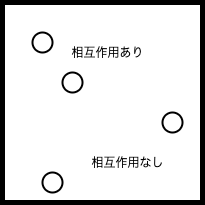
\includegraphics[width=6cm]{fig/middledensity.png}
    \end{center}
    \caption{中密度状態における分子の状態の概念図}
    \label{fig:middledensity.png}
\end{figure}

\newpage
流体相から固体相への相転移近傍の中密度状態では、相転移により圧力の振る舞いが急激に変化すると考えられる。
相転移近傍の中密度状態での数密度$\rho$とMDシミュレーションで測定されたWCAポテンシャルの圧力$P$の関係を
以下の図\ref{fig:middleden_den-pre}に示す。

\begin{figure}[htbp]
    \begin{center}
        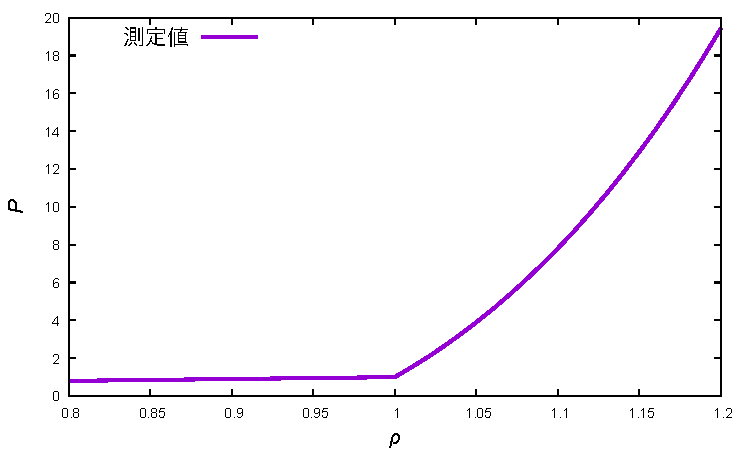
\includegraphics[width=14cm]{fig/middleden_den-pre.pdf}
    \end{center}
    \caption{WCAポテンシャルにおける中密度状態の数密度と圧力の関係}
    \label{fig:middleden_den-pre}
\end{figure}


図\ref{fig:middleden_den-pre}から$\rho\,{\simeq}\,1$付近で相転移が起こり、圧力の振る舞いが急激に変化することを確認できた。
この相転移の存在により、圧力の振る舞いが急激に変化するので、WCAポテンシャルの状態方程式を\ref{method-subsec:virial}節で示したビリアル展開や、
\ref{method-subsec:BWR}節で示したBWR,m-BWR方程式を用いて表すと項の個数が際限なく増え、項自体の物理的意味も不明瞭になると考えられる。


\subsection{高密度状態のWCAポテンシャルの圧力}\label{results-subsec:WCA-press-high-density}
高密度状態では、すべての分子ペアが相互作用を持つものと近似できる。
まず、高密度状態における分子の状態の概念図を以下の図\ref{fig:highdensity.png}に示す。

\begin{figure}[htbp]
    \begin{center}
        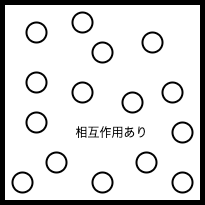
\includegraphics[width=6cm]{fig/highdensity.png}
    \end{center}
    \caption{高密度状態における分子の状態の概念図}
    \label{fig:highdensity.png}
\end{figure}

原子間の相互作用の寄与が大きい高密度状態では、圧力は式(\ref{eq:Theoritical-pressure})の第二項の影響を強く受ける。
高密度状態では、
密度が高くなればなるほど、式(\ref{eq:Theoritical-pressure})の第二項で考慮するものは、再隣接原子の寄与、第二隣接原子の寄与、第三隣接原子の寄与・・・と増えていく。

WCAポテンシャルにおいて原子間に働く力$\vec{r_{ij}}$の大きさは、
WCAポテンシャルのポテンシャルエネルギーが式(\ref{eq:wca})に従うことから、

\large
\begin{equation}
    | {\vec{r_{ij}}} |=\frac{d}{dr}\left(4\left(\left(\frac{1}{r}\right)^{12}-\left(\frac{1}{r}\right)^6\right)\right)=| 48r^{-13}-24r^{-7} |\label{eq:power}
\end{equation}
\normalsize
と書くことができるため、式(\ref{eq:Theoritical-pressure})の第二項の

\large
\begin{equation}
    \sum_{i=j}^N\vec{q_{ij}} \cdot \vec{r_{ij}} \label{eq:}
\end{equation}
\normalsize
は、距離に対して6乗で減衰することがわかる。

以上から、式(\ref{eq:Theoritical-pressure})の第二項への寄与はほとんどが再隣接原子であることから、本研究では、再隣接原子の寄与のみを考えるものとする。
第五隣接原子の寄与が生じる密度は、第五隣接原子間距離がWCAポテンシャルのカットオフ距離$2^{\frac{1}{6}}{\approx}1.12246$と等しい、すなわち
$\rho\,{\simeq}\,14.7$と表される。
これより高密度の状態では、次々に原子間の相互作用が働いていくが、この高密度状態でも圧力が式(\ref{eq:Theoritical-pressure})において
再隣接原子の寄与のみを考慮したもので十分に表されることを確認する。

式(\ref{eq:ideal-value})において再隣接原子の寄与のみを考慮したものを「理論近似値」、本研究におけるMDシミュレーションにより測定された圧力を「測定値」とし、その結果を図\ref{fig:highden_compare:den-pre}に示す。

\begin{figure}[htbp]
    \begin{center}
        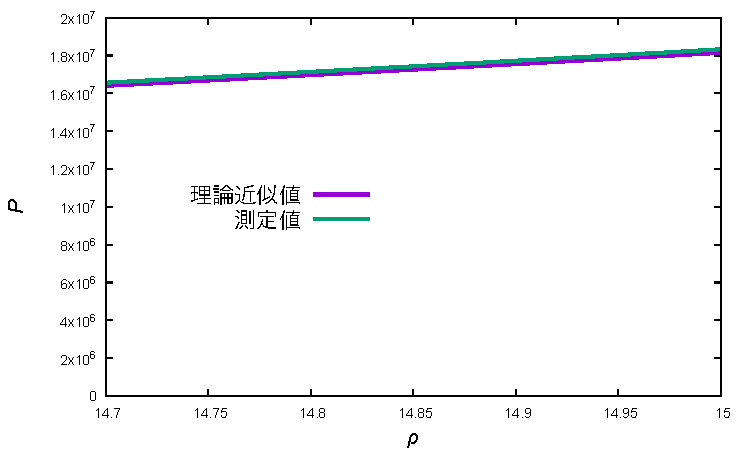
\includegraphics[width=14cm]{fig/highden_compare:den-pre.pdf}
    \end{center}
    \caption{WCAポテンシャルにおける高密度状態の圧力の理論近似値と測定値の比較}
    \label{fig:highden_compare:den-pre}
\end{figure}

図\ref{fig:highden_compare:den-pre}から、理論値と測定値のズレは1.2%以下であることがわかる。
このことから、第五隣接原子より離れた原子とも相互作用が働くほど高密度の状態でもWCAポテンシャルの圧力は式(\ref{eq:Theoritical-pressure})において
再隣接原子の寄与のみを考慮したもので十分に表されていることがわかる。



以上から、MDシミュレーションにより測定されたWCAポテンシャルの圧力の振る舞いを
原子間の相互作用をほぼ無視できる低密度状態、流体相から固体相への相転移近傍の中密度状態、原子間の相互作用の寄与が大きい高密度状態において確認できた。



\section{WCAポテンシャルの状態方程式}\label{results-sec:WCA-equation}
\ref{results-sec:WCA-press}節で示した圧力を数密度を含む項で展開することを試みたとき、\ref{method-subsec:virial}節で示したビリアル展開、
\ref{method-subsec:BWR}節で示したBWR,m-BWR方程式を用いると、\ref{results-subsec:WCA-press-middle-density}節で示した相転移の存在により、
項の個数が際限なく増え、項自体の物理的意味も不明瞭になると考えられる。
そこで、\ref{results-sec:WCA-equation}節では、\ref{results-sec:WCA-press}節で示したWCAポテンシャルにおける圧力と数密度の関係に上記で示した最小二乗法を適用し、
圧力を数密度に関する低次の多項式で近似することにより、WCAポテンシャルの状態方程式を推定する。

まず、本研究で得られたMDシミュレーションによる圧力の値を「測定値」、gnuplotを用いて5次式の最小二乗法を行った関数を「5次式近似」とし、
以下の図\ref{fig:5den-pre}に示す。


\begin{figure}[htbp]
    \begin{center}
        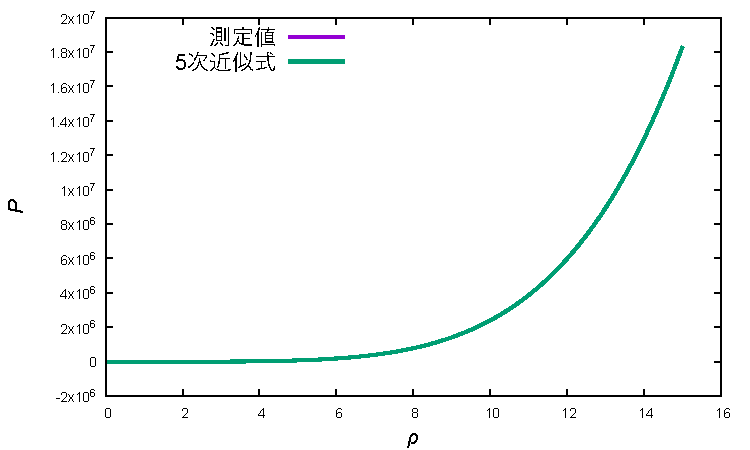
\includegraphics[width=14cm]{fig/5den-pre.pdf}
    \end{center}
    \caption{WCAポテンシャルの状態方程式の5次式近似}
    \label{fig:5den-pre}
\end{figure}



\section{ガウス過程回帰によるWCAポテンシャルの状態方程式の効率的推定}
ガウス過程回帰の過程

ガウス過程回帰とランダムサンプリングの精度の差?


\section{図の入れ方}

図は、数が多くなければとりえあずfigといったディレクトリにまとめて入れておくと良いだろう。数が増えてきて管理が難しくなったら節ごとにわけるなど工夫すること。画像ファイルは原則としてPDFにすること。例えば\verb|temperature.pdf|を入れたいなら、

\begin{lstlisting}[language=TeX]
    \begin{figure}[htbp]
        \begin{center}
            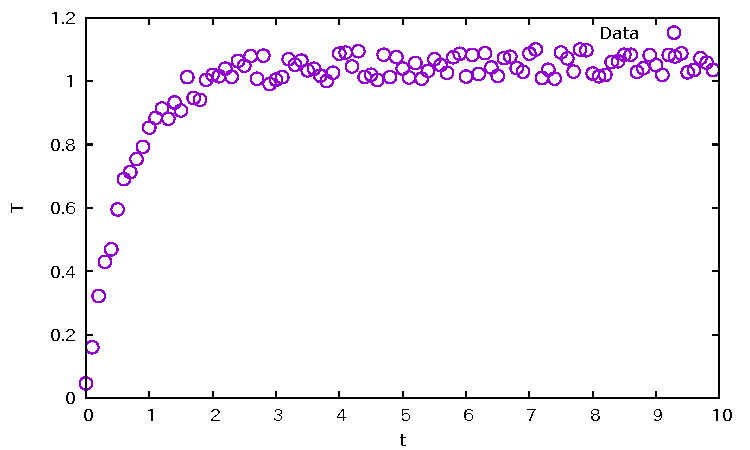
\includegraphics[width=10cm]{fig/temperature.pdf}
        \end{center}
        \caption{温度の時間発展。}
        \label{fig:temperature}
    \end{figure}
\end{lstlisting}

とすると、以下のような図が得られる。

\begin{figure}[htbp]
    \begin{center}
        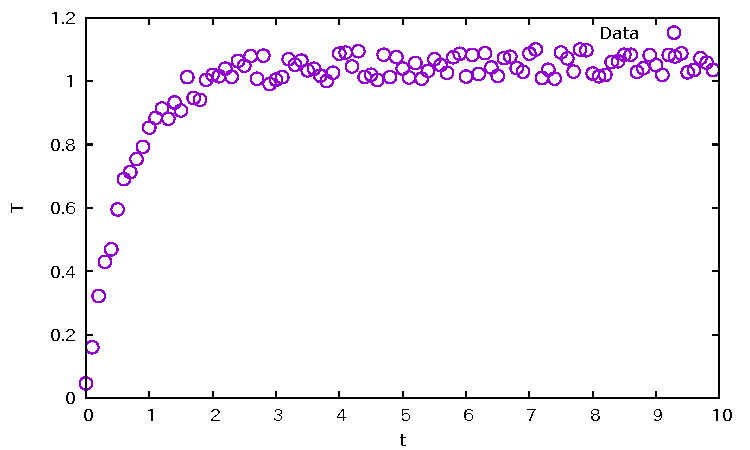
\includegraphics[width=10cm]{fig/temperature.pdf}
    \end{center}
    \caption{温度の時間発展。}
    \label{fig:temperature}
\end{figure}

この時、元データと、データからPDFを作るためのプロットファイルもしくはスクリプトファイルを一緒に入れておく。この時、画像ファイルとプロットファイルの名前を同じにしておくと良い。例えばgnuplotを使って\verb|temperature.pdf|という画像を作るなら、プロットファイルを\verb|temperature.plt|にしておく。すると、

\begin{lstlisting}[language=bash]
gnuplot temperature.plt
\end{lstlisting}

を実行することで\verb|temperature.pdf|ができるのでわかりやすい。

また、名前を揃えておくとmakefileとの相性が良くなる。例えば\verb|pressure.pdf|、\verb|temperature.pdf|、\verb|error.pdf|の三つのファイルが、同名のpltファイルから作成されるなら

\lstinputlisting[language=make]{fig/makefile}

といったmakefileを作っておけば、make一発で三つのファイルを作ることができるので便利だ。

もちろんPythonのMatplotlibを使っても良いが、いずれにせよ「データとスクリプトからコマンド一発で図のファイルが作成できる状況にしておく。

\chapter{考察および結論} \label{chap:summary}

考察は、「研究の背景」及び「目的」において提起した問題に正しく答えるようにする。得られた結果は満足すべきものだったか?不満があるならその理由はなにか?解決できそうなのか?また、「大きい理由」にも言及する。本研究によりどのような課題が見つかったかを書き、この分野における「研究の流れ」においてのような位置づけにあるかを説明した上で、今後、どのような発展の方向があるかについて書く。

\chapter*{謝辞}

まず、私を研究室に迎えれていただき、研究を進める上で、基礎的な部分から複雑な部分まで多くの指導をしていただいた渡辺宙志准教授には大変感謝しております。
研究部分のみならず、私たちの様子を常に気にかけ、研究設備や生活面でのサポートもしていただきましたこと心より御礼申し上げます。

また、同じ研究室に所属していた藤田くん、四辻くん、佐藤くんは、同じ部屋で研究を進め、分からない部分をお互いに共有しながら共に切磋琢磨できたと思います。
研究の合間に、昼ごはんを食べにいったり、他愛もない話をしたりと、息抜きをしながら研究を進めることが出来ましたこと、深く感謝致します。

最後に、研究のみならず、学生生活を様々な面でサポートしてくださった両親に深く感謝致します。


\appendix

\chapter{ソースコード}

\lstinputlisting[caption = 適当なPythonスクリプト, label = prog:sample]{src/sample.py}

\bibliographystyle{junsrt}
\bibliography{reference}

\end{document}